\documentclass[11pt,letterpaper]{article}

% Packages
\usepackage[empty]{fullpage}
\usepackage{hyperref}
\usepackage[left=0.5in,top=0.35in,right=0.5in,bottom=0.35in]{geometry}
\usepackage{titlesec}
\usepackage{enumitem}
\usepackage{xcolor}
\usepackage{fontawesome}
\usepackage{tabularx}
\usepackage{tikz}

% Define forest green color
\definecolor{forestgreen}{RGB}{34,139,34}
\definecolor{lightgreen}{RGB}{190,255,190}
\definecolor{darkgray}{RGB}{52,58,64}

% Colors for hyperlinks
\hypersetup{
    colorlinks=true,
    linkcolor=forestgreen,
    filecolor=forestgreen,
    urlcolor=forestgreen,
}

\parindent=0pt

% Custom section formatting
\titleformat{\section}
{\Large\scshape\raggedright\color{forestgreen}}
{}{0em}
{}[\titlerule]
\titlespacing*{\section}{0pt}{6pt}{3pt}

% Section heading without underline (rule)
\newcommand{\sectionnorule}[1]{
    \vspace{6pt}
    {\Large\scshape\raggedright\color{forestgreen}#1\par}
    \vspace{3pt}
}
% Custom commands
\newcommand{\tech}[1]{\textcolor{darkgray}{\textbf{#1}}}
\newcommand{\skill}[1]{{\small\textcolor{forestgreen}{\textbf{#1}}}}
\newcommand{\employer}[3]{
    \vspace{8pt}
    {\large\textcolor{forestgreen}{\textbf{#1}}}
    {\normalsize\textcolor{forestgreen}{—}}
    {\normalsize\textcolor{forestgreen}{{#2}}}
    \hfill
    {\normalsize\normalfont\mdseries\textcolor{forestgreen}{#3}}
    \par
}
\newcommand{\role}[2]{\hspace{1em}{\large\textcolor{forestgreen}{\textbf{#1}}} \hfill \textit{#2}}
\newcommand{\noproject}[1]{
    \hspace*{1em}{\small\color{darkgray}#1}
    \par
}
\newcommand{\project}[2]{
    \vspace{4pt}
    \hspace*{4pt}{\normalsize\textcolor{darkgray}{\textbf{#1}}}
    {\small\color{darkgray}
    \begin{itemize}[leftmargin=2em,itemsep=0pt,topsep=0pt,parsep=0pt,partopsep=0pt]
        #2
    \end{itemize}}
    \vspace{0pt}
    \par
}
\newcommand{\volunteer}[3]{
    \hspace*{1em}{\normalsize\textcolor{darkgray}{#1}}
    \textbf{—}
    \hspace*{0em}{\small\textcolor{darkgray}{#2}}
    \hfill
    #3
    \par
}

% Custom bullet points
\renewcommand{\labelitemi}{$\bullet$}

% Begin document
\begin{document}

% Header
\begin{center}
{\huge \textcolor{forestgreen}{\textbf{Andrew Gurik}}}\\[3pt]
    {\normalsize
    \textcolor{forestgreen} \faEnvelope\ andrewgurik@gmail.com
    \textcolor{forestgreen} \faGithub\ \href{https://github.com/gurellia53/resume}{\textcolor{darkgray}{github.com/gurellia53}}
    \textcolor{forestgreen} \faPhone\ (309) 868-4405
    \textcolor{forestgreen} \faMapMarker\ Ames, IA}\\[3pt]
\end{center}

Software Engineer with 12 years of experience in embedded software and controls. Most recently building precision agriculture software systems using modern C++ and Qt frameworks.

% Core Competencies
\sectionnorule{Core Competencies}
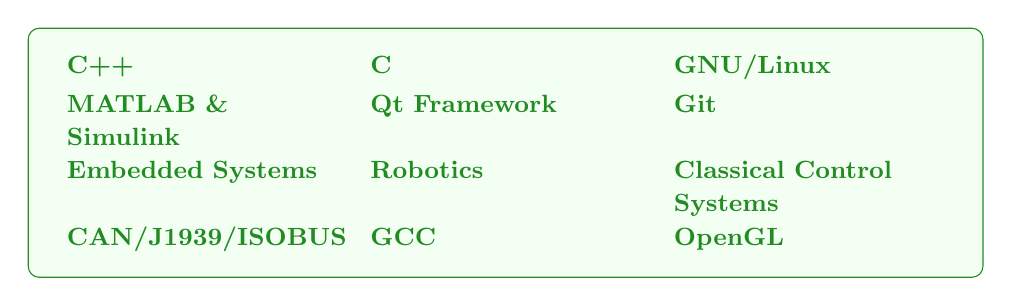
\begin{tikzpicture}
\node[rectangle,draw=forestgreen,rounded corners,inner sep=8pt,fill=lightgreen!20,text width=\dimexpr\textwidth-16pt\relax] {
\begin{tabularx}{\textwidth}{XXX}
\skill{C++} & \skill{C} & \skill{GNU/Linux} \\[2pt]
\skill{MATLAB \& Simulink} & \skill{Qt Framework} & \skill{Git} \\[2pt]
\skill{Embedded Systems} & \skill{Robotics} & \skill{Classical Control Systems} \\[2pt]
\skill{CAN/J1939/ISOBUS} & \skill{GCC} & \skill{OpenGL}
\end{tabularx}
};
\end{tikzpicture}

% Experience Section
\section{Experience}
\employer{Ag Leader Technology}{Staff Software Engineer}{2018 -- Present}
\noproject{Currently developing vision-based vehicle automation on an embedded NVIDIA Jetson platform.}
\project{In-Cab Touchscreen Display -- InCommand Go}{
    \item Led development of next-generation precision agriculture displays, implementing a 3D mapping engine using Qt3D and OpenGL in an embedded Linux environment (i.MX8 QM).
    \item Integrated a new 3D map engine with a legacy codebase while improving graphics performance.
    \item Developed custom OpenGL ES shaders to improve rendering performance and user experience.
}
\project{Liquid Application Control -- L2 \& RightSpot}{
    \item Developed a proprietary liquid application control system for precision agriculture sprayers.
    \item Designed the CAN protocol for third-party nozzle-by-nozzle control integration.
    \item Implemented closed-loop pressure and flow control for servo and PWM valves.
    \item Implemented nozzle duty-cycle controller using nozzle flow feed-forward and flow meter feedback.
    \item Integrated with OEM vehicles over J1939 and built simulators to validate and accelerate vehicle integration.
}
\project{High Speed Planting -- SureSpeed}{
    \item Developed a high-speed planting system using BLDC motors (seed meter and seed tube) and seed sensors communicating over J1939.
    \item Implemented touch-based in-cab diagnostics to improve troubleshooting and operator workflow.
    \item Used a modified hardware platform while preserving compatibility with existing features such as hydraulic downforce, clutch shutoffs, and advanced seed monitoring.
}
\employer{Randstad Technologies}{Software Engineer}{2017 -- 2018}
\project{Caterpillar -- Core Machine Software}{
    \item Built a desktop harness to run and debug embedded modules on a Windows PC.
    \item Integrated Windows DLLs with Simulink, custom C\#/C++ tooling, GTest, and a virtual CAN bus.
}
\employer{Caterpillar, Inc.}{Software Engineer}{2013 -- 2016}
\project{Drivetrain Systems \& Software -- Large Mining Trucks \& Off Highway Trucks}{
    \item Delivered features and bug fixes for powershift transmission control software in C and Simulink across legacy and new product lines.
    \item Maintained existing features using hydraulic solenoid control, J1939 communication, and speed sensor inputs while validating behavior with hardware-in-loop and software-in-loop testing.
}
% Volunteer Section
\section{Volunteer Experience}
\employer{FIRST Robotics Competition}{Mentor}{}
\volunteer{Team Neutrino, Story County 4H}{Lead Mentor (Controls)}{2012, 2020 -- Present}
\volunteer{Robot Casserole}{Mechanical Design Mentor}{2013 -- 2016}
% Education Section
\section{Education}
\employer{Iowa State University}{B.S. Electrical Engineering}{Fall 2012}
\end{document}
